\setcounter{section}{62}
\section{Алгоритм Борувки: выбор минимального ребра из нескольких, корректность, реализация, асимптотика.}

    Алгоритм Борувки - алгоритм поиска минимального остового (неориентированного) дерева на связанном неориентированном графе.
    
    Занумеруем рёбра графа начиная с единицы.
    
    \textbf{Алгоритм.} 
      
    Начало:
    
    1) Изначально в лесу каждое дерево – одна вершина. Каждая вершина --- отдельное дерево.
        
    Итерация:
    
    1) Для каждого дерева $T_i$ из леса $T$ выбираем самое легкое ребро, соединяющее $T_i$ с остальным графом. Добавляем найденные ребра в лес, объединяя связанные им деревья. 
    
    Замечание: 
    
    Важно аккуратно выбирать минимальные рёбра для каждого дерева, чтобы в случае, когда из вершин исходит несколько рёбер наименьшего веса, не возникла ситуация, как на первой картинке (появился цикл). Избежать проблемы возможно, если из наименьших рёбер выбирать ребро с минимальным номером. 

    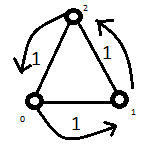
\includegraphics[scale=1]{images/63-71_1.png}
    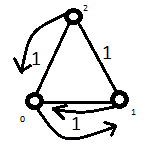
\includegraphics[scale=1]{images/63-71_2.png}
        
    \textbf{Теорема.} Алгоритм Борувки корректен.

    \textbf{Доказательство.}
    
    \parbox[t]{0.95\linewidth}{
        \begin{itemize}
            \item Будет построено дерево. Предположим, что это не так. (Будем проводить каждое неориентированное ребро от дерева, в котором оно выбрано, ко второй вершине.) 
            
            1) Предположим на некотором шаге будет построен простой цикл (хотя бы на 3-х вершинах), рёбра в котором были построены в одном направлении цикла (как пример - первая картинка выше). Если в цикле рёбра разной длины, то найдётся дерево, в котором было выбрано не минимальное по длине ребро. Если в цикле рёбра одной длины, то найдётся дерево, для которого было выбрано ребро большего номера, чем то, которое в него пришло. Противоречие. 
            
            2) Предположим результат алгоритма будет несвязным. Так как на каждом шаге алгоритма добавляется количество ребер равное $n$ - количеству деревьев в лесу. Рёбра не образуют циклов, а мест, где произошли совпадения рёбер не более $\frac{n}{2}$. (Если было проведено 2 ребра между двумя компонентами, то эти рёбра совпадают) Следовательно, на каждом шаге было проведено не менее $\frac{n}{2}$ различных рёбер, значит количество деревьев в лесу на каждом шаге уменьшалось как минимум в два раза. Следовательно, в итоге мы получим связный граф.
            
            Доказали, что будет построено дерево.
            
            \item Будет построено дерево минимального веса. От противного. По аналогии с теоремой о разрезе рассмотреть первое добавленное ребро, не принадлежащее мин.остову.
        \end{itemize}
    }
    
    \textbf{Утверждение.} Алгоритм Борувки работает за $O(E log V)$
    
    \textbf{Доказательство.} На каждом шаге количество деревьев уменьшается не менее чем в 2 раза. Следовательно, количество итераций не больше $log V$. Один шаг выполняется за $O(E)$. Общее время работы ---  $O(E log V)$. \qed

\setcounter{section}{63}
\section{Определение паросочетания в произвольном графе, двудольного графа, увеличивающего пути.}

        \textbf{Определение.} Двудольный граф --- это граф, множество вершин которого можно разбить на две части таким образом, что каждое ребро графа соединяет каждую вершину из одной части с какой-то вершиной другой части, то есть не существует рёбер между вершинами одной и той же части графа.

      \textbf{Определение.} Паросочетание в (обычном неориентированном) графе - произвольное множество ребер, такое что никакие два ребра не имеют общей вершины.
    
      \textbf{Определение.} Паросочетание $M$ в двудольном графе - произвольное множество рёбер двудольного графа, такое что никакие два ребра не имеют общей вершины.
      
      \textbf{Определение.} Вершина $v$ насыщена (инцидентна, покрыта) ребрами из паросочетания M, если $v$ лежит в одном из рёбер $M$. Остальные вершины называются ненасщенными (свободными). 
    
      \textbf{Определение.} Рёберное покрытие графа — множество рёбер, в котором каждая вершина графа инцидентна по меньшей мере одному ребру покрытия.
    
      \textbf{Определение.} \textit{Максимальное} паросочетание~--- это паросочетание в графе $G$, содержащее максимальное количество ребер
    
      \textbf{Определение.} Паросочетание называется совершенным(полным), если оно покрывает все вершины графа
      
      \textbf{Определение.} Цепь (путь) - последовательность вершин, в которой каждая вершина соединена со следующей ребром.
    
      \textbf{Определение.} Чередующаяся цепь (путь) - цепь в двудольном графе, для любых двух соседних рёбер которой верно, что одно из них принадлежит паросочетанию, а другое нет
    
      \textbf{Определение.} Увеличивающая (дополняющая) цепь (путь) в $G$ относительно паросочетания $M$ - чередующаяся цепь, у которой оба конца свободные вершины.
      
    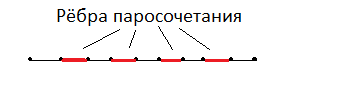
\includegraphics[scale=1.5]{images/63-71_цепь.png}
    

\setcounter{section}{64}
\section{Лемма об устройстве неориентированного графа, в котором степени всех вершин не превосходят двух.}

    \textbf{Лемма.} Неориентированный граф, в котором степени всех вершин не превосходят двух, состоит из цепей и циклов.
    
    Доказывается проходом по графу:
    
    Если есть вершины степени 1, то начинаем идти по рёбрам начиная с неё, когда-то придём к концу (мы рассматриваем лишь конечные графы), получили цепь. Если все вершины степени 2, то начинаем идти по рёбрам начиная с некоторой вершины, так как наш проход не может закончится ни на одной другой вершине, ведь их степень 2 и граф конечный, то проход замкнётся на той вершине, с которой мы начинали. Получили цикл. 
    
    В итоге получим, что граф состоит из простых путей и циклов.

\setcounter{section}{65}
\section{Теорема Бержа.}

    \textbf{Теорема.}(Бержа) Паросочетание M в двудольном графе $G$ является максимальным тогда и только тогда, когда в $G$ нет дополняющей цепи.
    
    \textbf{Доказательство.}
    
        $\Rightarrow$
    
        Пусть в двудольном графе $G$ с максимальным паросочетанием $M$ существует дополняющая цепь. Тогда пройдя по ней и заменив вдоль неё все рёбра, входящие в паросочетание, на не входящие и наоборот, мы получим большее паросочетание. То есть $M$ не являлось максимальным. Противоречие.
            
        $\Leftarrow$
        
        От противного. Пусть $M$ – не максимальное. Пусть $M’$ – другое паросочетание, $|M'| > |M|$. Рассмотрим их симметрическую разницу. В таком графе все вершины имеют степень не больше 2 (т.е. все компоненты будут цепями или циклами). Найдется компонента, в которой ребер $M’$ больше. Это будет увеличивающей цепью для $M$, а не циклом, так как в цикле всегда одинаковое количество рёбер из $M$ и $M'$. (Потому что любое ребро цикла принадлежит либо $M$, либо $M'$ и в цикле чётное число рёбер) А это противоречие к условию отсутствия для $M$ увеличивающих цепей.

\setcounter{section}{66}
\section{Алгоритм Куна. Корректность, реализация, асимптотика.}

    \textbf{Алгоритм Куна.}
    
        Задан граф $G\langle V, E \rangle$, про который известно, что он двудольный, но разбиение не задано явно. Требуется найти наибольшее паросочетание в нём
        
        Алгоритм можно описать так: сначала возьмём пустое паросочетание, а потом — пока в графе удаётся найти увеличивающую цепь, — будем выполнять чередование паросочетания вдоль этой цепи, и повторять процесс поиска увеличивающей цепи. Как только такую цепь найти не удалось — процесс останавливаем, — текущее паросочетание и есть максимальное.
        
        В массиве $\mathtt{matching}$ хранятся ребра паросочетания: $ (v, \mathtt{matching}[v]) $ ($v$ - вершина левой доли, $\mathtt{matching}[v]$ - вершина правой доли) (Если паросочетания с вершиной $ v $ не существует, то $ \mathtt{matching}[v]= -1$). А $used$ — обычный массив "посещённостей" вершин в обходе в глубину (он нужен, чтобы обход в глубину не заходил в одну вершину дважды).
        Функция $ \mathrm{dfs} $ возвращает  $true$, если ей удалось найти увеличивающую цепь из вершины $v$, при этом считается, что эта функция уже произвела чередование паросочетания вдоль найденной цепи.
        
        Внутри функции $dfs(v)$, где $v$ - вершина левой доли, просматриваются все рёбра, исходящие из вершины $v$, и затем проверяется: если это ребро ведёт в ненасыщенную вершину $ to$, то возвращаем true. Если эта вершина $to$ насыщена, но удаётся найти увеличивающую цепь рекурсивным запуском из $\mathtt{matching}[to]$ (т.е. $dfs(\mathtt{matching}[to]) = true)$, то мы говорим, что мы нашли увеличивающую цепь. Производим чередование в текущем ребре: перенаправляем ребро, смежное с $to$, в вершину $v$, возвращаем $true$.
        
        В основной программе сначала указывается, что текущее паросочетание — пустое (массив $ \mathtt{matching}$ заполняется числами $-1$). Затем перебирается все вершины левой доли, и из них запускается обход в глубину $ \mathrm{dfs}$, предварительно обнулив массив $used$. 
        
\textbf{Немного корректности:}

Из теоремы в следующем билете следует, что если из вершины $x$ не существует увеличивающей цепи относительно паросочетания $M$, тогда из $x$ не существует увеличивающей цепи в $M'$ (паросочетание $M'$ получается из $M$ изменением вдоль увеличивающей цепи).

Следовательно, если от вершины $v$ запускался хоть раз dfs, то из $v$ больше никогда нельзя будет провести удлиняющую цепь.

Так как любая удлиняющая цепь имеет концы в разных долях, то после запуска dfs из всех вершин левой доли в графе не останется удлиняющих цепей. Следовательно, мы получим максимальное паросочетание. 

\textbf{Реализация:}
        
\begin{lstlisting}
bool dfs(int м) {
    if (used[v]) return false;
    used[v] = true;
    for (to : g[v]) {
        if (matching[to] == -1 || dfs(matching[to])) {
            matching[to] = v;
            return true; 
        }
    }
    return false;
}
 	
int main() {
    matching.assign(n, -1); \\ где n - количество вершин левой доли. 
    for (int i = 0; i < n; ++i) {
        used.assign(n, false);
        dfs(i);
    }
    for (int i = 0; i < n; ++i) {
      	if (matching[i] != -1) {
           	cout << i << " " << matching[i] << endl;
        }
    }
}
\end{lstlisting}

\textbf{Асимптотика:}

        Можно явно задано разбиение графа размера $n$ на две доли размером $n_1$ и $n_2$. Алгоритм Куна можно представить как серию из $n_1$ запусков обхода в глубину на всём графе.
        Следовательно, всего этот алгоритм исполняется за время $O(n_1m)$ (или $O(nm)$), где $m$ {{---}} количество рёбер.


\setcounter{section}{67}
\section{Лемма об отсутствии увеличивающих путей из вершины при отсутствии таких путей относительного меньшего паросочетания.}

        \textbf{Теорема.}  Если из вершины $x$ не существует увеличивающей цепи относительно паросочетания $M$, тогда из $x$ не существует увеличивающей цепи в $M'$ (паросочетание $M'$ получается из $M$ изменением вдоль увеличивающей цепи).
        
        \textbf{Доказательство.}
        
        Доказательство от противного.

        Допустим в паросочетание внесли изменения вдоль дополняющей цепи $(y \rightsquigarrow z)$ (цепь из $y$ в $z$) и из вершины $x$ появилась дополняющая цепь.
        Заметим, что эта дополняющая цепь должна вершинно пересекаться с той цепью, вдоль которой вносились изменения, иначе такая же дополняющая цепь из $x$ существовала и в исходном паросочетании.
        
        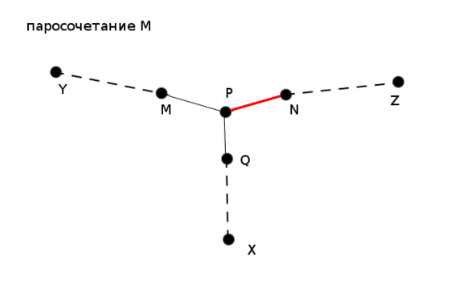
\includegraphics[scale=1]{images/63-71_Kuhn2}
        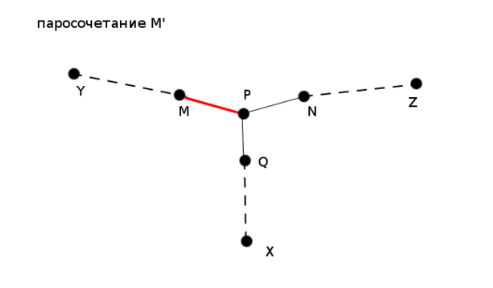
\includegraphics[scale=1]{images/63-71_Kuhn1}
        
        Пусть $p$ – ближайшая к $x$ вершина, которая принадлежит и новой дополняющей цепи и цепи $(y \rightsquigarrow z)$.
        Тогда $MP$ – последнее ребро на отрезке $(y \rightsquigarrow p)$ цепи $(y \rightsquigarrow z)$, $NP$ – последнее ребро на отрезке $(z \rightsquigarrow p)$ цепи $(y \rightsquigarrow z)$, $QP$ - последнее ребро лежащее на отрезке $(x \rightsquigarrow p)$ новой дополняющей цепи.
        
        Допустим $MP$ принадлежит паросочетанию $M'$, тогда $NP$ ему не принадлежит.
        (Случай, когда $NP$ принадлежит паросочетанию $M'$ полностью симметричен.)
        
        Поскольку паросочетание $M'$ получается из $M$ изменением вдоль дополняющей цепи $(y \rightsquigarrow z)$, в паросочетание $M$ входило ребро $NP$, а ребро $MP$ нет.
        Кроме того, ребро $QP$ не лежит ни в исходном паросочетании $M$, ни в паросочетании $M'$, в противном случае оказалось бы, что вершина $p$ инцидентна нескольким рёбрам из паросочетания, что противоречит определению паросочетания.
        
        Тогда заметим, что цепь $(x \rightsquigarrow z)$, полученная объединением цепей $(x \rightsquigarrow p)$ и $(p \rightsquigarrow z)$, по определению будет дополняющей в паросочетании $M$, что приводит к противоречию, поскольку в паросочетании $M$ из вершины $x$ не существует дополняющей цепи. (по условию задачи)
        



\setcounter{section}{68}
\section{Определения независимого множества, вершинного покрытия. Связь определений.}

\textbf{Определение.} Подмножество вершин графа $G$ называется независимым множеством, если не существует ребра графа соединяющего какие-либо две из них.

\textbf{Определение.} Подмножество вершин графа $G$ называется вершинным покрытием $G$, если любое ребро графа содержит вершину из этого множества.

\textbf{Связь.} Подмножество вершин является независимым множеством тогда, и только тогда когда его дополнение является вершинным покрытием. 

(лемма следует из определения)

\textbf{Утверждение.} Подмножество вершин является максимальным независимым множеством тогда, и только тогда когда его дополнение является минимальным вершинным покрытием.

\setcounter{section}{69}
\section{Алгоритм поиска максимального независимого множества и минимального вершинного покрытия в двудольном графе с помощью разбиения на доли $L^-; L^+;R^-;R^+$ (с доказательством).}

Пусть $G$ - двудольный неориентированный граф, в нём $M$ - максимальное паросочетание. Строим $D$ - граф $G$, в котором рёбра из $M$ ориентированы справа налево, а остальные слева направо. Пусть $L, R$ - множество вершин левой и правой доли соответственно. Запустим обход из всех ненасыщенных вершин левой доли. Пусть $L^-$ - посещённые обходом вершины левой доли, $L^+$ - не посещённые вершины левой доли. Для правой доли аналогично. Тогда 
$$L^- \cup R^+ - \text{минимальное вершинное покрытие}$$
$$L^+ \cup R^- - \text{максимально независимое множество}$$

\textbf{Корректность:}

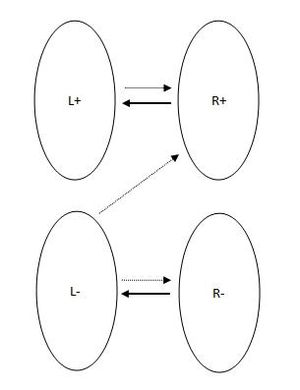
\includegraphics[scale=0.5]{images/63-71_пути2}

Понятно, что не могут быть рёбра из $L^+$ в $R^-$ и из $R^+$ в $L^-$. Также нет рёбер из $R^-$ в $L^+$. Предположим противное и существует такое ребро из $u$ в $v$. Это ребро ведёт справа налево, следовательно, оно из $M$, тогда $v$ насыщена и из неё не запускали обход, но $v$ была посещена ($v \in L^+$). Следовательно, существует путь до $v$ из какой-нибудь ненасыщенной вершины левой доли $w$. Но единственный способ попасть в вершину $v$ из правой доли это ребро $(u, v)$. При этом вершина $v$ была посещена обходом, а $u$ нет ($u \in R^-$). Противоречие. Следовательно, нет рёбер из $R^-$ в $L^+$  

По картинке видно, что $L^+ \cup R^- - \text{независимое множество}$, а $L^- \cup R^+ - \text{вершинное покрытие}$.

Осталось доказать, что $L^- \cup R^+ - \text{минимальное вершинное покрытие}$. Покажем, что $|L^- \cup R^+| \leq |M|$:

1) В $L^-$ лежат только насыщенные паросочетанием $M$ вершины.

2) В $R^+$ лежат только насыщенные вершины (иначе есть увеличивающий путь)

3) $\forall (u, v) \in M: u \not \in L^-$ или $v \not \in R^+$.

Показали.

Покажем, что мощность вершинного покрытия не меньше мощности максимального паросочетания:

Понятно, что каждое ребро $M$ будет покрыто хотя бы одной вершиной из вершинного покрытия.

Показали оценку снизу, показали оценку сверху. Cледовательно, $|VC| \geq |M| \geq |L^- \cup R^+| \geq |VC|$, где $VC$ - минимальное вершинное покрытие. 
Следовательно,
$$L^- \cup R^+ - \text{минимальное вершинное покрытие}$$
$$L^+ \cup R^- - \text{максимально независимое множество}$$

\setcounter{section}{70}
\section{Алгоритм поиска максимального независимого множества и минимального вершинного покрытия в двудольном графе с помощью задачи 2SAT.}

В предыдущем доказательстве мы показали, что мощность минимального вершинного покрытия (МВП) равна мощности максимального паросочетания (МП), т.е. |МВП| = |МП|. Следовательно, каждая вершина из МВП лежит на ребре максимального паросочетания и ровно одна на каждом ребре. Зададим на каждом ребре порядок: одна вершина ребра - левая, другая - правая. Значит нам необходимо решить задачу: какую вершину каждого ребра МП нужно выбрать для МВП. Пронумеруем рёбра паросочетания. Введём обозначения: переменная $x_1 = 1$, если вершина МВП может быть правой вершиной первого ребра максимального паросочетания, и  $x_1 = 0$, если вершина МВП может быть левой вершине ребра. Для остальных рёбер максимального паросочетания вводим аналогичные переменные. Далее для каждого ребра графа выписываем логическую формулу, так чтобы в любой ситуации удовлетворяющей формуле хотя бы одна вершина МВП покрыла данное ребро:

1) Например, если ребро соединяет две насыщенные вершины одна из которых правая вершина ребра $i$-го ребра МП, а другая левая вершина ребра $j$-го ребра МП, то формула будет выглядеть как: $x_i \vee \overline{x_j}$

2) Если ребро имеет только одну насыщенную вершину - правую вершину $i$-го ребра МП. Формула будет выглядеть как: $x_i$

3) Если у ребра нет насыщенных вершин, то её можно включить в паросочетание. Противоречие с максимальностью паросочетания.

Получили систему логических формул, решив которую получим искомое минимальное вершинное покрытие. Систему можно решить с помощью алгоритма 2SAT. Свели.